% !TEX root = ../thesis.tex


\chapter{Methods}
\label{cha:dmd_methods}
In this chapter, I am first going to describe the optical setup that was built to work on the DMD independently from the running experiment. To use a camera for image correction with the DMD, a pixel to pixel mapping is needed. For this, I will start with the algorithm to calibrate the camera and then explain how this calibration is used to map a camera image to DMD pixel coordinates. Finally, I will introduce the actual error correction algorithms.

\section{Testing Setup}
\label{sec:dmd_testing_setup}
Figure~\ref{fig:dmd_test_setup} shows the test setup that was built for the development of the correction algorithms. We use a \SI{770}{nm} laser\footnote{Toptica DL Pro} as illumination for the DMD\footnote{Vialux DLP7000}. The beam is guided onto the table with an optical fibre and then collimated by a lens with a long focal length. The large diameter beam is then reflected onto The DMD with a mirror mounted on a rotation mount. The angle of this mirror is adjusted such that the \emph{ON}-direction of the DMD is level with the breadboard while the \emph{OFF}-direction is shown onto a beam dump. The projection is then imaged onto a CCD camera\footnote{Thorlabs DDC1545M, monochrome sensor, $1280\times 1024$ pixels} with a microscope.
\begin{figure}[htbp]
    \centering
    \tikzset{mynode/.style={draw=black,solid,circle,fill=white,inner sep=2pt}}
\begin{tikzpicture}
    \node[anchor=south west, inner sep=0] (image) at (0,0,0) {\includegraphics[width=.67\textwidth,trim=0 0 0 75px,clip]{DMD/TestSetup/DSC_3218}};
    \begin{scope}[x={(image.south east)},y={(image.north west)}]
        \node[mynode](fibre) at (0.67,0.81){\scriptsize A};
        \node[mynode](beamexpander1) at (0.4,0.65){\scriptsize B};
        %\node[mynode](beamexpander2) at (0.54,0.76){B};
        \node[mynode](dmd) at (0.77,0.68){\scriptsize C};
        \node[mynode](beamdump) at (0.87,0.51){\scriptsize D};
        \node[mynode](telescope1) at (0.44,0.39){\scriptsize E};
        \node[mynode](telescope2) at (0.71,0.33){\scriptsize E};
        \node[mynode](camera) at (0.81,0.41){\scriptsize F};
    \end{scope}
\end{tikzpicture}
    \caption[Test setup for the DMD]{Test setup for the DMD. The laser beam from the optical fibre (A) is collimated by a lens (B) and then mirrored onto the DMD (C). A beam dump (D) captures the excess light in the \emph{OFF}-direction. The light reflected in the \emph{ON}-direction is imaged onto the CCD camera (F) using a microscope (E).}
    \label{fig:dmd_test_setup}
\end{figure}

\section{Camera Calibration}
\label{sec:dmd_camera_calibration}
As mentioned earlier, a good camera calibration is needed for usable correction results. The better we know which camera pixels are related to which DMD pixels, the more accurate we can make the correction algorithm. A very simple idea would be to take the positions of the DMD corners on the camera and then apply a rectangular transformation to get the mapped coordinates. But due to nonlinear imaging aberrations, the DMD edges could appear slightly curved on the camera. This makes a simple rectangular transformation generally impractical. While the setup in this work could indeed function with only a rectangular transformation between camera and DMD, the algorithms developed here are supposed to function in a general scenario.

So instead, we project a pattern of small dots which we can detect on the camera. If the distance between these dots is small enough, the edges they form can be approximated as straight lines, even if the line between two corners of the image is curved. The quadrilaterals formed by four dots can be mapped to the corresponding square on the DMD using an algorithm that conserves the ratio between two lengths (see section \ref{sec:dmd_mapping}). We further require the number of dots in both directions to be odd so the centre of the DMD has a dot in all cases.

\subsection*{Point Detection}
% \label{sec:dmd_point_detection}
Figure~\ref{fig:point_matrix_example} shows the camera image of a grid of points with equal spacing. Although the edges of the pattern projected from the DMD are dark, the camera captures a lot of reflected light from the edges of the DMD chip. For calibration, we can easily circumvent this by taking another picture where all pixels are set to OFF and subtracting this from the image with the points.
\begin{figure}[htbp]
    \centering
    \pdfpxdimen=\dimexpr 1 in/96\relax
    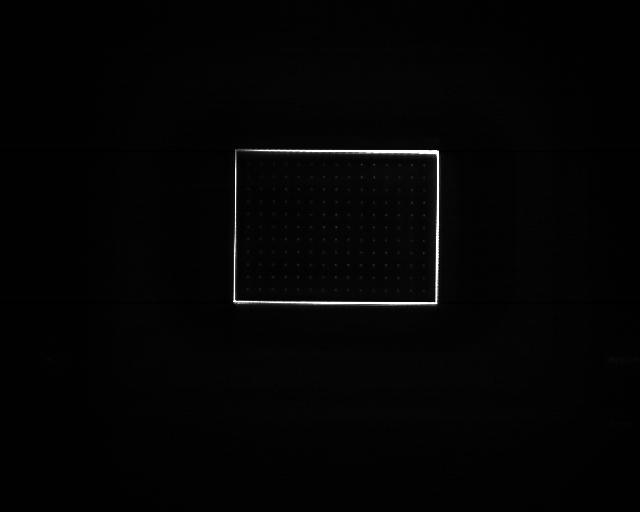
\includegraphics[scale=1.4,trim=220px 194px 186px 140px,clip]{DMD/grid-unmapped}
    \caption[Camera image of a grid with 165 equally spaced points]{Camera image of a grid with equally spaced points. The original image is $640\times 512$ pixels large, the image shown here has been cropped to the region $220,140$~--~$454,318$ ($244\times 178$).}
    \label{fig:point_matrix_example}
\end{figure}
The detection algorithm for the points works as follows:
\begin{enumerate}
    \item Iterate over all the pixels from top to bottom and left to right.
    \item If the intensity at one pixel reaches a previously fixed threshold, search the region \SI{5}{px} in all directions for the pixel with the highest intensity $(x_\text{max},y_\text{max})$.
    \item The coordinates of the gridpoint are determined as an intensity-weighted average over the region \SI{5}{px} around $(x_\text{max},y_\text{max})$: \[\begin{pmatrix}
        x \\ y
    \end{pmatrix} = \frac{\sum\limits_{j = -5}^5 \sum\limits_{i = -5}^5 \begin{pmatrix}
        x_\text{max} + i \\ y_\text{max} + j
    \end{pmatrix}\times I(x_\text{max} + i, y_\text{max} + j)}{\sum\limits_{j = -5}^5 \sum\limits_{i = -5}^5 I(x_\text{max} + i, y_\text{max} + j)} \]
    \item The region that has been searched in step 2 and the region over which the average is taken in step 3 are marked as processed. This ensures that the same gridpoint is not \enquote{detected} twice.
\end{enumerate}
% To detect the points on the camera image, the pixels are traversed from top to bottom and from left to right  and if a pixel reaches a certain intensity, the region around this pixel is searched for the brightest spot. The location of the point is then decided by intensity-weighted averaging over a region aroung the brightest pixel (Alg.~\ref{alg:dmd_point_detection}).
%
All gridpoints that have been detected are added to a common list. Unfortunately, this list is not necessarily sorted, meaning it is not yet possible to assign a point from the original grid to one corresponding point in the list of detected points. 

\subsection*{Point Sorting}
% \label{sec:dmd_point_sorting}
We sort the detected gridpoints from the centre outwards (see Figure~\ref{fig:sorting_tikz}). 
\begin{figure}[htbp]
    \centering
    \usetikzlibrary{shapes.misc}
\tikzset{blackdot/.style={shape=circle,fill=black,scale=0.35}}
\tikzset{missing/.style={shape=circle,scale=0.35}}
\tikzset{newdot/.style={shape=circle,fill=progression1,scale=0.4}}
\tikzset{founddot/.style={shape=circle,fill=progression0,opacity=0.8,scale=0.35}}
\tikzset{cross/.style={cross out, draw=black, minimum size=2*(#1-\pgflinewidth), inner sep=0pt, outer sep=0pt, line width=0.8pt},
cross/.default={3pt}}
\tikzstyle{arrow} = [thick,->,>=stealth, line width=0.8pt]
\tikzstyle{greyarrow} = [thick,->,>=stealth,color=black,opacity=0.6,line width=0.8pt]
\newcounter{cnti}
\begin{tikzpicture}[scale=0.525,yscale=-1]
    \foreach \xoffset in {0,1,2,3,4}
    \foreach \yoffset in {0,1}
    \foreach \x in {0,...,4}
    \foreach \y in {0,...,4}
    {
        \ifnum\numexpr(\xoffset + 5*\yoffset - 10)*(\xoffset + 4*\yoffset - 11)\relax=0
        \else
            \ifnum\numexpr\x + 5*\y\relax=22
                \setcounter{cnti}{\number\numexpr1+\xoffset + 5*\yoffset\relax}
                \node[blackdot,label={[label distance=.5ex]below:{\textbf{\footnotesize(\alph{cnti})}}}] (\x-\y-\xoffset\yoffset) at (\x + 6.5*\xoffset,\y + 6.5*\yoffset){};
            \else
                \ifnum\numexpr(\x + 5*\y - 6)*(\x + 5*\y - 19)\relax=0
                    \node[missing] (\x-\y-\xoffset\yoffset) at (\x + 6.5*\xoffset,\y + 6.5*\yoffset){};
                \else
                    \node[blackdot] (\x-\y-\xoffset\yoffset) at (\x + 6.5*\xoffset,\y + 6.5*\yoffset){};
                \fi
            \fi
        \fi
    }
    \foreach \mnode in {%
        2-1-00,2-3-00%
        ,2-0-10,2-4-10%
        ,1-2-20,3-2-20%
        ,1-1-30,3-1-30,1-3-30,3-3-30%
        ,1-0-40,1-4-40,3-0-40,3-4-40%
        ,0-2-01,4-2-01%
        ,0-1-11,0-3-11,4-1-11,4-3-11%
        ,0-0-21,0-4-21,4-0-21,4-4-21%
        }
    {
        \draw (\mnode) node[newdot]{};
    }
    \foreach \mnode in {%
        1-1-40,1-1-01,1-1-11,1-1-21,1-1-31,4-3-21,4-3-31,4-3-41%
        }
    {\draw (\mnode) node[cross]{};}
    \foreach \mnode in {%
        2-2-00%
        ,2-2-10,2-1-10,2-3-10%
        ,2-2-20,2-1-20,2-0-20,2-3-20,2-4-20%
        ,2-2-30,2-1-30,2-0-30,2-3-30,2-4-30,1-2-30,3-2-30%
        ,2-2-40,2-1-40,2-0-40,2-3-40,2-4-40,1-2-40,3-2-40,3-1-40,1-3-40,3-3-40%
        ,2-2-01,2-1-01,2-0-01,2-3-01,2-4-01,1-2-01,3-2-01,3-1-01,1-3-01,3-3-01,1-0-01,1-4-01,3-0-01,3-4-01%
        ,2-2-11,2-1-11,2-0-11,2-3-11,2-4-11,1-2-11,3-2-11,3-1-11,1-3-11,3-3-11,1-0-11,1-4-11,3-0-11,3-4-11,0-2-11,4-2-11%
        ,2-2-21,2-1-21,2-0-21,2-3-21,2-4-21,1-2-21,3-2-21,3-1-21,1-3-21,3-3-21,1-0-21,1-4-21,3-0-21,3-4-21,0-2-21,4-2-21,0-1-21,0-3-21,4-1-21%
        }
    {
        \draw (\mnode) node[founddot]{};
    }
    \foreach \start/\end in {%
    2-2-00/2-1-00,2-2-00/2-3-00%
    ,2-1-10/2-0-10,2-3-10/2-4-10%
    ,2-2-20/1-2-20,2-2-20/3-2-20%
    ,1-2-30/1-1-30,1-2-30/1-3-30,3-2-30/3-1-30,3-2-30/3-3-30%
    ,1-1-40/1-0-40,1-3-40/1-4-40,3-1-40/3-0-40,3-3-40/3-4-40%
    ,1-2-01/0-2-01,3-2-01/4-2-01%
    ,0-2-11/0-1-11,0-2-11/0-3-11,4-2-11/4-1-11,4-2-11/4-3-11%
    ,0-1-21/0-0-21,0-3-21/0-4-21,4-1-21/4-0-21,4-3-21/4-4-21%
    }
    {
        \draw [arrow] (\start) -- (\end);
    }
    \foreach \start/\end in {%
    2-2-10/2-1-10,2-2-10/2-3-10%
    ,2-2-30/2-1-30,2-2-30/2-3-30%
    ,1-2-40/1-1-40,1-2-40/1-3-40,3-2-40/3-1-40,3-2-40/3-3-40%
    ,2-2-01/1-2-01,2-2-01/3-2-01%
    ,1-2-11/1-1-11,1-2-11/1-3-11,3-2-11/3-1-11,3-2-11/3-3-11%
    ,0-2-21/0-1-21,0-2-21/0-3-21,4-2-21/4-1-21,4-2-21/4-3-21%
    }
    {
        \draw [greyarrow] (\start) -- (\end);
    }
    \foreach \xy in {%
        0-0,1-0,2-0,3-0,4-0%
        ,0-1,2-1,3-1,4-1%
        ,0-2,1-2,2-2,3-2,4-2%
        ,0-3,1-3,2-3,3-3%
        ,0-4,1-4,2-4,3-4,4-4%
    }
    {
        \draw (\xy-31) node[founddot]{};
    }
    \foreach \start in {1-0,0-1,2-1,1-2}
    {\draw [arrow] (\start-31) -- (1-1-31);}
    \foreach \xy in {%
        0-0,1-0,2-0,3-0,4-0%
        ,0-1,1-1,2-1,3-1,4-1%
        ,0-2,1-2,2-2,3-2,4-2%
        ,0-3,1-3,2-3,3-3%
        ,0-4,1-4,2-4,3-4,4-4%
    }
    {
        \draw (\xy-41) node[founddot]{};
    }
\end{tikzpicture}
    \caption[Sketch of the point sorting algorithm]{Sketch of the point sorting algorithm. The central column is handled first and then the rows are expanded outwards. All detected grid points are black, already sorted ones blue and currently searched ones red. The black arrows are pointing to the estimated location of the next gridpoint and the grey arrows show the local basis vectors. Missing gridpoints are indicated by a cross.}  
    \label{fig:sorting_tikz}
\end{figure}
\begin{enumerate}
    \item Find the basis vectors from the central gridpoint up ($\hat{y}$) and to the right ($\hat{x}$) by projecting two more images with only the centre and one neighbouring spot in the vertical and horizontal direction lit up respectively. 
    \item Use $\hat{y}$ and $-\hat{y}$ to find the nearest points up and down from the centre. \textbf{(a)}
    \item Continue up and down, using the difference between the last two points to define new local basis vectors $\hat{y}_\uparrow$ and $\hat{y}_\downarrow$. \textbf{(b)}
    \item Stop at the gridpoints closest to the edges.
    \item Expand to the columns to the right and left from the centre, using $\hat{x}$ and $-\hat{x}$ to locate the nearest gridpoints left and right. \textbf{(c)}
    \item To find the next points up and down, use the difference between the already found gridpoints one column inwards to get an estimate. \textbf{(d)}
    \item Continue up and down as in step 3 and 4, defining now four different local basis vectors $\hat{y}_{\uparrow,l}, \hat{y}_{\uparrow,r}, \hat{y}_{\downarrow,l}, \hat{y}_{\downarrow,r}$. \textbf{(e)}
    \item Missing gridpoints are replaced by the respective guess \textbf{(e)}, \textbf{(h)}; See below for detail.
    \item Repeat steps 5~--~7 until all the gridpoints except the outermost edges have been sorted. \textbf{(f)}~--~\textbf{(h)}
    \item If possible, improve the estimated position of missing points \textbf{(i)}; See below for detail.
\end{enumerate}
In each step, the actual coordinates of the gridpoint are found from the estimated position $P_\text{guess}$ by searching the detected list for the closest match $\tilde{P}$. Until now, the underlying assumption has been that all gridpoints have actually been detected in the previous stage. However, if that is not the case, the point $\tilde{P}$ might be a neighbouring gridpoint. To account for this, the distance between $P_\text{guess}$ and $\tilde{P}$ must not exceed half the distance between the last two known gridpoints. Otherwise, the point is marked as \enquote{missing} and replaced by $P_\text{guess}$ for the time being, just to be able to continue with the sorting \textbf{(e)},\textbf{(h)}. At the end, missing gridpoints can be replaced by averaging the coordinates of the gridpoints to the left, right, top and bottom, but only if those have not been marked as missing themselves \textbf{(i)}. 
If too many points are missing, the entire list is rejected and the calibration fails.

Finally, we have to address the gridpoints at the outer edges. Due to the leakage light as seen in Figure~\ref{fig:point_matrix_example}, points at the edges can never be detected and have to be extrapolated at the end of the sorting algorithm. This extrapolation can lead to errors in the mapping, which are very apparent in the example in Figure~\ref{fig:mapping_example_mapped}.

% The vertical basis vector is used to find the next point up- and downwards from the centre. Now the next points are found using the difference between the last two points as a guess:
% \begin{equation}
%     P_{n+1,\text{guess}} = 2P_n - P_{n-1} \nonumber
% \end{equation}
% Once a column has been completely sorted, the horizontal basis vector is used to find the starting points of the next column (step 3) etc.\ until all points are sorted.

% To get the actual coordinates of a grid point from the guess, the list of detected points is searched for the point with the smallest distance to $P_{n+1,\text{guess}}$. If this distance too high, it is likely that a neighboring point was selected and the target point had not been detected at all. If this happens, the guess is used instead. The grid positions of these points is stored in a separate list. When all grid points are sorted, either by finding the correct point in the list of detected points or by guessing, we can try to improve all the guesses. If the surrounding four points (left, right, top and bottom) of a guessed point have been detected correctly, the guessed one is updated as the average of these four surrounding points. If the number of remaining guesses is too high after this, the complete list is rejected. Because the edges of the DMD appear very bright on the camera, the outermost points are all guesses. This is of course not ideal and results in errors which can be seen in Fig.~\ref{fig:mapping_example_mapped}.

Of course, the need for a sorting method like this could be avoided entirely if every single gridpoint was projected by itself. However, this can take very long and if the calibration works reliably while needing far fewer images, then the added complication is worth it.

\section{Camera Mapping}
\label{sec:dmd_mapping}
At this point we know the coordinates of the camera pixels that correspond to the gridpoints on the DMD. Now we need to find an expression for all the pixels in between. We can reduce this problem to a singular square of gridpoints on the DMD. We know the coordinates of the four pixels on the camera that mark the corners of this square, therefore we can map the space inbetween them using the scheme shown in Fig.~\ref{fig:dmd_mapping_scheme}.
\begin{figure}[hbp]
    \centering
    \begin{tikzpicture}[scale=1]
    \tikzmath{\z = 3;}
    \draw (0,0) node[label={[label distance=-2*\z pt]225:{$C(0|1)$}}] (bl) {} --
    (\z,0) node[label={[label distance=-2*\z pt]315:{$D(1|1)$}}] (br) {} --
    (\z,\z) node[label={[label distance=-2*\z pt]45:{$B(1|0)$}}] (tr) {} --
    (0,\z) node[label={[label distance=-2*\z pt]135:{$A(0|0)$}}] (tl) {} -- cycle;
    \path[name path=uDmd] ($(bl)!0.3!(br)$) -- ($(tl)!0.3!(tr)$);
    \path[name path=vDmd] ($(bl)!0.4!(tl)$) -- ($(br)!0.4!(tr)$);
    \draw[name intersections={of=uDmd and vDmd,by={P}},densely dotted] ($(bl)!0.4!(tl)$) -- (P) node [midway,below] {$x$};
    \draw[densely dotted] ($(tl)!0.3!(tr)$) -- (P) node [midway,right]{$y$};
    \node[label={[label distance=-3*\z pt]315:{$P(x|y)$}}] at (P) {};

    \draw [-{Latex[length=3mm]}] (\z*1.4,\z/2) -- (\z*2.1,\z/2);
    \draw (2.5*\z + 0.1*\z,0) node[label={[label distance=-2*\z pt]225:{$C'$}}] (C) {} --
    (2.5*\z+1.2*\z,0) node[label={[label distance=-2*\z pt]315:{$D'$}}] (D) {} --
    (2.5*\z+\z,\z*1.15) node[label={[label distance=-2*\z pt]45:{$B'$}}] (B) {} --
    (2.5*\z,\z) node[label={[label distance=-2*\z pt]135:{$A'$}}] (A) {} -- cycle;
    \path[name path=uCam] ($(C)!0.3!(D)$) -- ($(A)!0.3!(B)$);
    \path[name path=vCam] ($(C)!0.4!(A)$) -- ($(D)!0.4!(B)$);
    \draw[name intersections={of=uCam and vCam,by={Pstar}},densely dotted] ($(A)!0.3!(B)$) -- (Pstar) node [midway, right] {$y'$};
    \draw[densely dotted] ($(C)!0.4!(A)$) -- (Pstar) node [midway, below] {$x'$};
    \node[label={[label distance=-3*\z pt]315:{$P'(x'|y')$}}] at (Pstar) {};
    \node[label={[label distance=-1.25*\z pt]270:{\scriptsize$W$}}] at ($(C)!0.3!(D)$) {};
    \node[label={[label distance=-1.25*\z pt]90:{\scriptsize$U$}}] at ($(A)!0.3!(B)$) {};
    \node[label={[label distance=-1.25*\z pt]0:{\scriptsize$V$}}] at ($(D)!0.4!(B)$) {};
    \node[label={[label distance=-1.25*\z pt]180:{\scriptsize$Z$}}] at ($(C)!0.4!(A)$) {};
\end{tikzpicture}
    \caption{Mapping a unit square onto an irregular quadrilateral}
    \label{fig:dmd_mapping_scheme}
\end{figure}
To find the coordinates of a point on an irregular quadrilateral $P'$ that corresponds to a point $P$ on a unit square, we take the $x$ and $y$ coordinates on the unit square and apply them as length ratios to the sides of the quadrilateral, $\overline{A'B'}$ and $\overline{C'D'}$ for the $x$ direction and $\overline{A'C'}$ and $\overline{B'D'}$ for the $y$ direction, giving us the points $U,V,W,Z$. The point $P'$ is found where the lines $\overline{UW}$ and $\overline{ZV}$ cross:
\begin{align}
    \overrightarrow{P'} &= \left\{ \overrightarrow{U} + r\cdot \left(\overrightarrow{W} - \overrightarrow{U}\right) \right\} \cap \left\{ \overrightarrow{Z} + s\cdot \left(\overrightarrow{V} - \overrightarrow{Z}\right) \right\} \nonumber
    \intertext{where}
    \overrightarrow{U} &= \left(\overrightarrow{A'} + x\cdot\overrightarrow{A'B'}\right), \quad \overrightarrow{W} = \left(\overrightarrow{C'} + x\cdot\overrightarrow{C'D'}\right) \nonumber \\
    \overrightarrow{Z} &= \left(\overrightarrow{A'} + y\cdot\overrightarrow{A'C'}\right), \quad \overrightarrow{V} = \left(\overrightarrow{B'} + y\cdot\overrightarrow{B'D'}\right) \nonumber
\end{align}
The coordinates $(x'|y')$ are then found as
\begin{align*}
    \begin{pmatrix}
        x' \\ y'
    \end{pmatrix} &= \overrightarrow{U} + r \cdot \left(\overrightarrow{W} - \overrightarrow{U}\right) 
    \intertext{with}
    r &= \frac{Z_y - U_y - (Z_x - U_x)\frac{V_x - Z_x}{V_x - Z_x}}{W_y - U_y - (W_x - U_x)\frac{V_y - Z_y}{V_x - Z_x}}.
\end{align*}
Applying this to the DMD, we get the following algorithm for mapping each individual pixel $P$:
\begin{enumerate}
    \item Find the closest four gridpoints and their corresponding camera counterparts.
    \item Use the scheme explained before to find the floating point coordinates $(x' | y')$ of this pixel on the camera $P'$.
    \item The mapped pixel value is then found by averaging the four pixels surrounding $P'$, with weights given by the reciprocal distance to $P'$: \[I_\text{mapped} = \frac{\sum\limits_{j=0}^1 \sum\limits_{i=0}^1 \frac{I_\text{camera}(\floor{\tilde{x}} + i,\floor{\tilde{y}} + j)}{\sqrt{\left(\floor{\tilde{x}} - \tilde{x} + i\right)^2 + \left(\floor{\tilde{y}} - \tilde{y} + j\right)^2}}}{\sum\limits_{j=0}^1 \sum\limits_{i=0}^1 \frac{1}{\sqrt{\left(\floor{\tilde{x}} - \tilde{x} + i\right)^2 + \left(\floor{\tilde{y}} - \tilde{y} + j\right)^2}}} \]
\end{enumerate}
Figure~\ref{fig:mapping_example} shows an example of the applied mapping algorithm.
% \textbf{Note:} Because the mapped coordinates of $P'$ are floating point values, the intensity on the mapped image is calculated from the average of the four pixels surrounding $P'$, weighted by the distance of the pixel to the floating point coordinates of $P'$. An example of the mapped camera image can be seen in Figure~\ref{fig:mapping_example}
\begin{figure}[htbp]
    \centering
    \begin{subfigure}[c]{0.5\textwidth}
        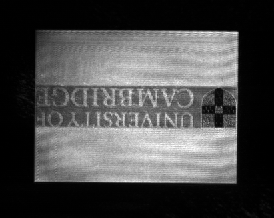
\includegraphics[width=\textwidth]{DMD/Mapping/camlogo2-unmapped}
        \caption{Unmapped camera image}
    \end{subfigure}\\ \vspace{1ex}
    \begin{subfigure}[c]{0.43\textwidth}
        \frame{
\includegraphics[width=\linewidth]{DMD/Mapping/camlogo2-target}}
        \caption{Target pattern on the DMD}
        \label{fig:mapping_example_target}
    \end{subfigure}
    \begin{subfigure}[c]{0.43\textwidth}
        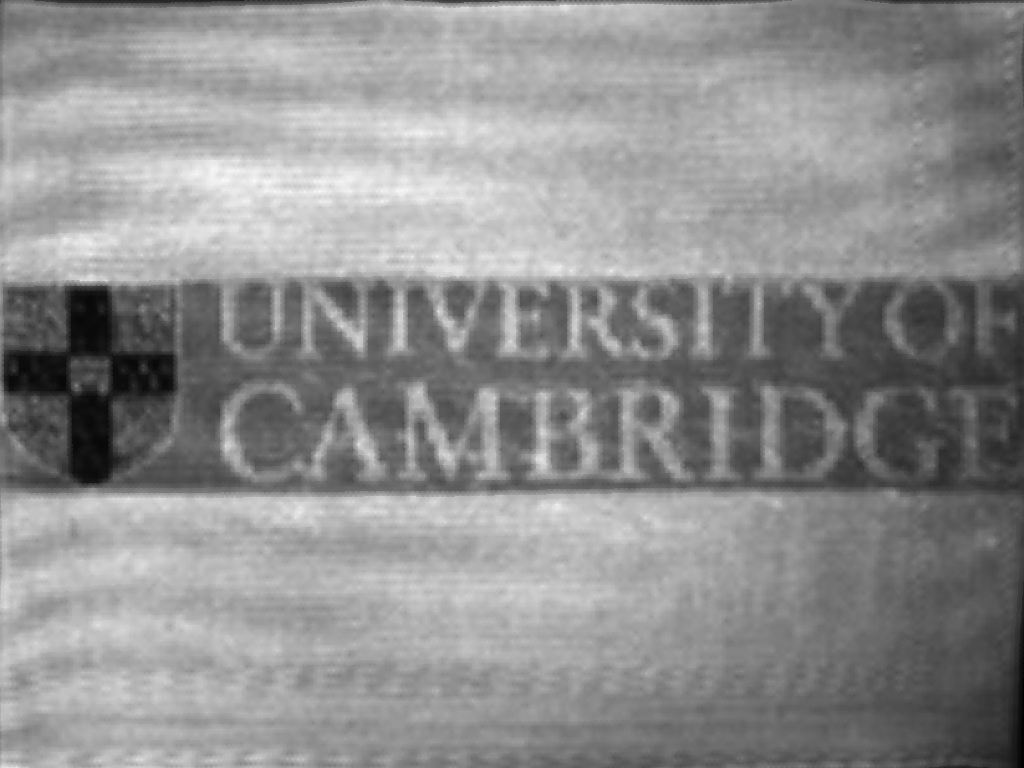
\includegraphics[width=\linewidth]{DMD/Mapping/camlogo2-mapped}
        \caption{Resulting mapped image}
        \label{fig:mapping_example_mapped}
    \end{subfigure}
    \caption[Example images for the camera-to-DMD mapping]{Example images for the camera-to-DMD mapping. The unmapped camera capture (cropped) is shown in (a). (b) and (c) show the comparison between the projected pattern and the mapped image. Note that the rotation of the camera image was corrected automatically.}
    \label{fig:mapping_example}
\end{figure}

\section{Error Correction}
\label{sec:dmd_error_correction_theory}
The previous works mentioned before were mainly concerned with the creation of flat-top beams. For this purpose, the entire dynamic range of the DMD was usable. However, if there is stray light in a portion where the DMD pixels are already off, it is not possible to reduce the light level in that area as a correction. This situation will be the main focus of the correction algorithms here.

The generation of an error signal is very straightforward. A camera image is taken and mapped. We can then subtract the target intensities from the pattern projected on the DMD\footnote{If the target was a grayscale image, the DMD pattern will have to be blurred by a small amount to reverse the dithering.} from this to get the intensity deviation. Figure~\ref{fig:imaging_error_example} shows an example of this. At the edges of the shapes, large errors are detected. These result from subpixel mapping errors and from the surrounding light. Because they would otherwise lead to strong overcorrections, these edge effects should be handled separately by the correction algorithm.
\begin{figure}[hbp]
    \centering
    \begin{subfigure}[t]{0.43\textwidth}
        \centering
        \frame{
\includegraphics[width=\linewidth]{DMD/Mapping/twoshapes-target}}
        \caption{DMD target pattern}
        \label{fig:imaging_error_target}
    \end{subfigure}
    \begin{subfigure}[t]{0.43\textwidth}
        \centering
        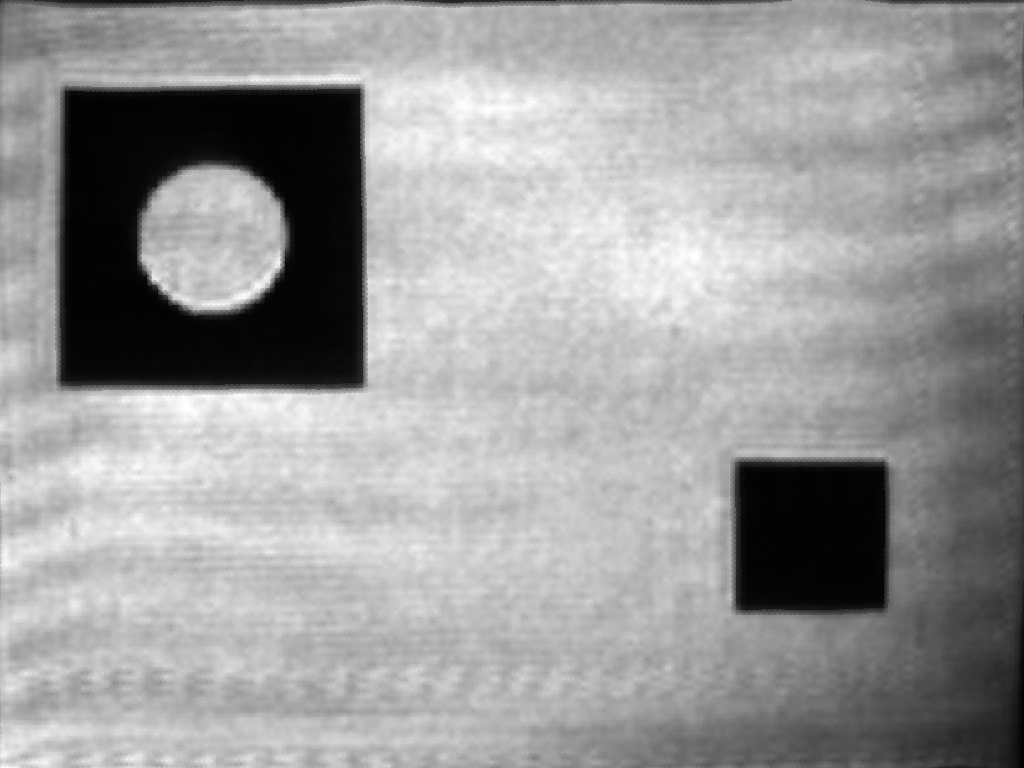
\includegraphics[width=\linewidth]{DMD/Mapping/twoshapes-mapped}
        \caption{Resulting mapped camera image}
    \end{subfigure} \\ \vspace{1ex}
    \begin{subfigure}[t]{\textwidth}
        \centering
        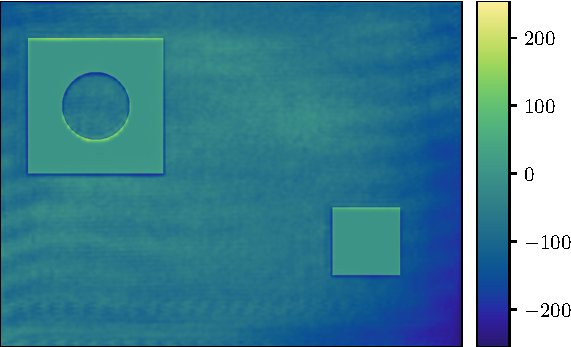
\includegraphics[]{DMD/Mapping/twoshapes-error}
        \caption{Intensity error ($\text{camera} - \text{target}$)}
    \end{subfigure}
    \caption[Example of DMD imaging error]{Example of DMD imaging error. At the edges of the shapes, large deviations are detected.}
    \label{fig:imaging_error_example}
\end{figure}

\subsection{Edge Detection}
To perform this edge detection, we can use a simple contrast-based model. We define an edge as a region where the difference of the intensity of neighboring pixels exceeds a certain threshold value. The discontinuinity $D$ in the vertical and horizontal direction at position $(x,y)$ is calculated as follows:
\begin{align*}
    D_\text{vertical}(x,y,r) &= \frac{\sum_{j=-r}^{r} \sum_{i=-r}^{r} \left| I_{x+i,y+j} - I_{x+i,y-j} \right|}{\sum_{j=-r}^{r} \sum_{i=-r}^{r} \chi (x+i,y+j,x+i,y-j)} \\
    D_\text{horizontal}(x,y,r) &= \frac{\sum_{j=-r}^{r} \sum_{i=-r}^{r} \left| I_{x+i,y+j} - I_{x-i,y+j} \right|}{\sum_{j=-r}^{r} \sum_{i=-r}^{r} \chi (x+i,y+j,x-i,y+j)}
\end{align*}
and there is an edge at $(x,y)$ if
\begin{equation*}
    D_\text{vertical} > D_\text{threshold} \lor D_\text{horizontal} > D_\text{threshold}
\end{equation*}
Here, $r$ is the radius of the square area around $(x,y)$ that is sampled over, $I_{i,j}$ is the intensity at pixel $(i,j)$ and $\chi(x_1,y_1,x_2,y_2)$ is defined as 1 if both points are within the image area and 0 otherwise. This algorithm has been adapted from Wu et al \cite{wu:2015}. 

$D_\text{threshold}$ and $r$ are user-specified parameters. In this work, $D_\text{threshold}$ was always fixed to a value of 35. A lower value results in the detection of far more pixels as edges and a higher value does not guarantee the detection of all edges. How the $r$ parameter has to be chosen depends on how well the DMD surface is resolved on the camera.This influence is studied in detail in Sec.~\ref{sec:results_edgedetection}.
Fig.~\ref{fig:edge_detection_example} shows the detected edges with a radius of $r=\SI{4}{px}$ in the patterns from Fig.~\ref{fig:imaging_error_example} and \ref{fig:mapping_example}.
\begin{figure}[htbp]
    \centering
    \begin{subfigure}[t]{0.43\textwidth}
        \centering
        \frame{
\includegraphics[width=\linewidth]{DMD/EdgeDetection/camlogo-edges-1pxblur}}
        \caption{Edges in Fig.~\ref{fig:mapping_example_target}}
    \end{subfigure}
    \begin{subfigure}[t]{0.43\textwidth}
        \centering
        \frame{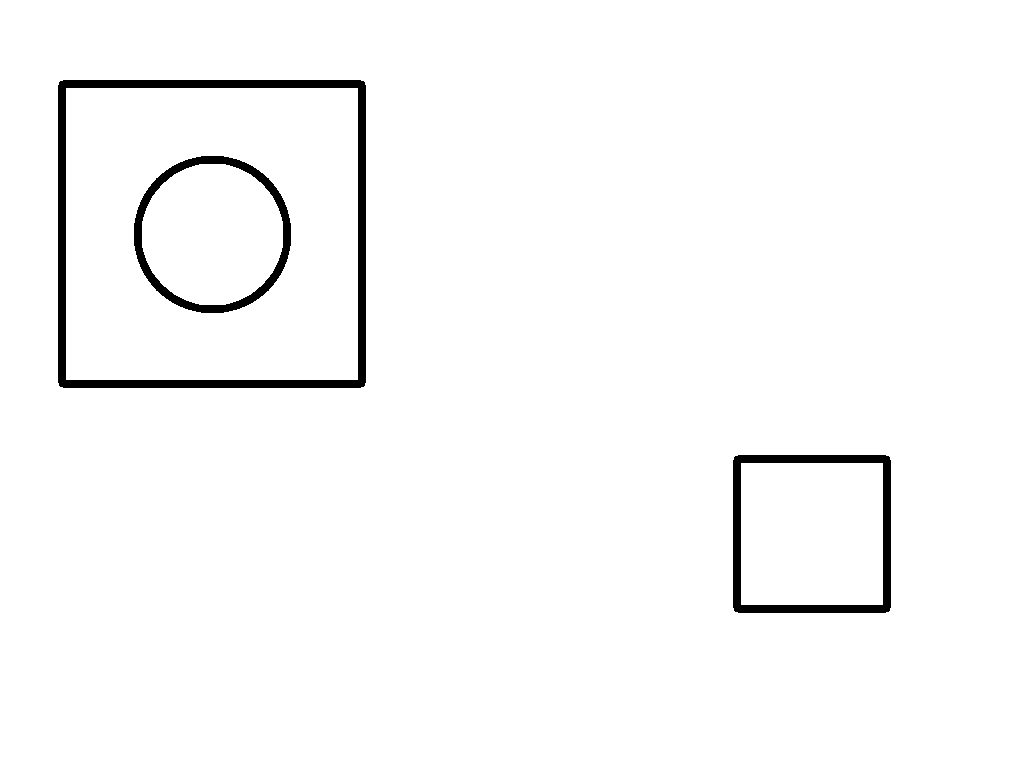
\includegraphics[width=\linewidth]{DMD/EdgeDetection/twoshapes-edges-noblur}}
        \caption{Edges in Fig.~\ref{fig:imaging_error_target}}
    \end{subfigure}
    \caption[Example of the edge detection algorithm]{Example of the edge detection algorithm. Note that the dithering in Fig.~\ref{fig:mapping_example_target} was reversed before applying the edge detection by using a gaussian blur filter with a \SI{1}{px} radius.}
    \label{fig:edge_detection_example}      
\end{figure}


\subsection{Linear Feedback}
The correction we are aiming for is directed both at the parts that are too dark and the parts that are too bright. If the target intensity in an area is 0 but there is actually light in that area, we obviously cannot reduce this light level using the DMD. Instead, we have to raise the overall light level so the deviation is evened out. Parts of the image that are too dark need to receive more light. If this is not possible because the DMD already reflects \SI{100}{\percent} of the incident light, then we have to reduce the overall light level. This is demonstrated in Fig.~\ref{fig:linear_feedback_scheme}.
\begin{figure}[hbp]
    \centering
    \begin{subfigure}[c]{0.52\textwidth}
        \centering
        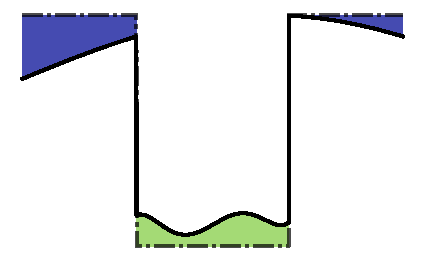
\includegraphics[]{DMD/LinearFeedbackSketch/sketch}
        \caption{Uncorrected}
    \end{subfigure}
    \begin{subfigure}[c]{0.47\textwidth}
        \centering
        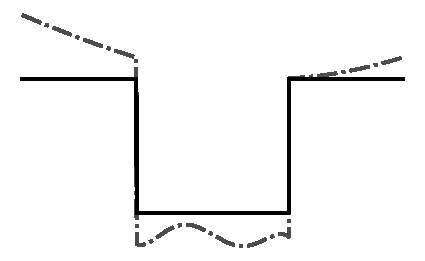
\includegraphics[]{DMD/LinearFeedbackSketch/sketch1_correct}
        \caption{Corrected}
    \end{subfigure}
    \caption[Basic example of the correction algorithm for a box]{Basic example of the correction algorithm for a box. Left side: the box pattern on the DMD (dashed-dotted) results in a camera image (solid) with deviations (blue $=$ too dark, red $=$ too bright). Assuming a linear relationship between DMD reflectivity and camera intensity, the corrected pattern on the right would result in a box with lower contrast but correct shape. The lower contrast would manifest itself in a reduced lifetime due to increased scattering of light in the centre.}
    \label{fig:linear_feedback_scheme}
\end{figure}

\noindent
We split the linear feedback into two parts. In the first iteration it is decided by how much the maximum intensity needs to be pulled down and how much of an offset needs to be introduced to the dark parts. The following iterations only serve to improve on the results of the first correction.
%
\begin{enumerate}
    \item Blur both the target pattern and the camera capture with a gaussian filter of \SI{1}{px} radius. The target needs to be blurred in this way because of the dithering that had been applied before. The mapped camera image is blurred to remove very fine noise that could not be corrected anyway as the mapping is not completely perfect on the single pixel level.
    \item Convert grayscale levels from the range $[0,255]$ to $[0,1]$
    \item Apply the edge detection on the target image and store the results as boolean values.
    \item Calculate the difference between camera and target brightness \[\Delta_{ij} = I_\text{Camera}[i,j] - I_\text{DMD}[i,j].\] For pixels that are at an edge, ignore the difference and set it to 0.
    \item Find the extrema of the difference. The positive maximum $\Delta^+$ is the amount by which the picture needs to be brightened and vice versa for the negative maximum $\Delta^-$. 
    \item Calculate the difference at the edges again. This time, do not ignore it, but use the extrema found before as limits.
    \item Calculate the updated pattern as \[I_\text{DMD}'[i,j] = I_\text{DMD}[i,j]\times \underbrace{(1- | \Delta^- | - \Delta^+)}_{\text{Rescaling}} + \underbrace{\Delta^+}_{\text{Offset}} - \Delta_{ij}. \] The rescaling and offset are applied to account for the reduced overall dynamic range. The updated image then has minimum and maximum values of $\Delta^+$ and $1 - |\Delta^-|$.
    \item Apply dithering and upload to the DMD.
    \item[] 
    \item Capture a new camera image and blur it as before (\SI{1}{px} gaussian).
    \item Calculate the difference to the target. Ignore values that are out of bounds.
    \item Update the target pattern, apply dithering and upload to the DMD.
    \item Repeat 9.~--~11.\ until the relative reduction of the RMS deviation of two subsequent images is less than \SI{2}{\percent}.
\end{enumerate}


\subsection{Maxima/Minima Suppression}
The second correction algorithm also uses the difference between camera and target as feedback, but it inherently uses the binary nature of the DMD. Rather than calculating a new pattern of grayscale values and dithering that again, it switches certain pixels on or off depending on the brightness values on the camera image. This method was originally developed by Liang et.\ al \cite{liang:2010}.
\begin{enumerate}
    \item Calculate the difference between camera and target. During this procedure, edges are ignored completely.
    \item Find the pixel with the maximum deviation (both positive and negative).
    \item Search the surrounding area for the nearest pixel that is neither too bright nor too dark. The search is performed on the edges of a square with side length $r$, where $r$ starts at 1 and increases until a pixel with a deviation of the opposite sign of the original pixel is found.
    \item Sum up the target and actual intensities $I_\text{target}$ and $I_\text{actual}$ of all the pixels in this area.
    \item Count the number of pixels on the DMD in this area that are already on $N_\text{\textit{ON}}$.
    \item The number of pixels that have to be switched is then given by \[N_\text{switch} = \left| \frac{I_\text{target}}{I_\text{actual}} - 1 \right|\times N_\text{\textit{ON}}. \]
    \item Switch on/off $N_\text{switch}$ pixels in this area. For this, draw pixel coordinates from a gaussian distribution centered around the pixel with maximum difference and with a standard deviation of half the side length of the square area used for the integral. If the pixel at the drawn coordinates does not need to be switched, draw new coordinates.
    \item Mark the area as \enquote{processed} by setting the difference to 0.
    \item Repeat steps 1.~--~7.\ until the whole image has been processed.
    \item Project the new pattern.
    \item Repeat until the RMS error of two subsequent images has shrunk by less than \SI{1.5}{\percent}.
\end{enumerate}
Unfortunately, because many points of deviation have rather small areas surrounding them where the sign of the difference stays the same, this adjustment process is very slow. We decided that it would be best to set additional breakoff conditions. One iteration is stopped if the number of pixels that has been switched on or off reaches a threshold value. This means that noise on the smallest scale is effectively ignored. Another breakoff condition is derived from the variance of the difference. Whenever the difference is set to 0 for a certain area (see above, step 8), this is also reflected in a theoretical change in the total variance. Once the square root of the variance (the RMS error) falls below a threshold, the search for new maxima and minima is stopped. Overall, we also put a limit on how often new maxima/minima are searched in the difference image. This last breakoff is mainly due to time constraints. All conditions are outlined in Table~\ref{tab:suppression_breakoffs}.
\begin{table}[htbp]
    \centering
    \begin{tabular}{rS[table-format=5]S[table-format=1.2]S[table-format=5]}
        \toprule
        \multicolumn{1}{c}{Iteration} & \multicolumn{1}{c}{max.\ ON/OFF switches} & \multicolumn{1}{c}{min.\ RMS error / \si{\percent}} & \multicolumn{1}{c}{\shortstack[c]{max.\ no.\ of maxima/\\ minima processed}}  \\
        \midrule
        1     & 20000 & 1 & 20000 \\
        2     & 10000 & .2 & 10000 \\
        $>2$  & 10000 & .01 & 40000 \\
        \bottomrule
    \end{tabular}
    \caption[Breakoff conditions for the maxima/minima suppression algorithm]{Breakoff conditions for the maxima/minima suppression algorithm.}
    \label{tab:suppression_breakoffs}
\end{table}
It is important to point out that the RMS error is \emph{not} the actual RMS error of the resulting image, just a helping variable used in the algorithm that tracks the \emph{remaining} error when the differences are set to 0 to indicate that an area has been processed.

\vspace{1ex}
\noindent
In this work, the linear feedback and the maxima/minima suppression algorithms are run successively. 